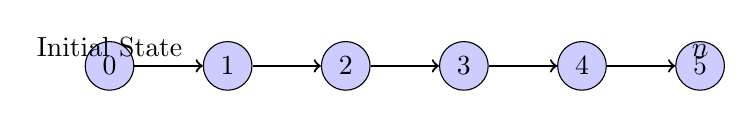
\begin{tikzpicture}
\foreach \n in {0,1,2,3,4,5} {
    \node[circle, draw, fill=blue!20] at (\n*1.5,0) (F\n) {$\F{\n}$};
}
\draw[->, thick] (F0) -- (F1);
\draw[->, thick] (F1) -- (F2);
\draw[->, thick] (F2) -- (F3);
\draw[->, thick] (F3) -- (F4);
\draw[->, thick] (F4) -- (F5);
\node[above] at (F0) {Initial State};
\node[above] at (F5) {$\U{n}$};
\end{tikzpicture}
